\documentclass{article} % This command is used to set the type of document you are working on such as an article, book, or presenation

\usepackage{geometry} % This package allows the editing of the page layout
\usepackage{amsmath}  % This package allows the use of a large range of mathematical formula, commands, and symbols
\usepackage{graphicx}  % This package allows the importing of images

\newcommand{\question}[2][]{\begin{flushleft}\textbf{Question #1}: \textit{#2}\end{flushleft}}
\newcommand{\sol}{\textbf{Solution}:} %Use if you want a boldface solution line
\newcommand{\maketitletwo}[2][]{\begin{center}
        \Large{\textbf{Homework 2 Report}
        
            Reinforcement Learning} % Name of course here
        \vspace{5pt}
        
        \normalsize{
            Name: Kai-Jie Lin 
            
            Student ID: 110652019
            
            \today}
        \vspace{15pt}
        \end{center}}
\begin{document}
    \maketitletwo[5]  % Optional argument is assignment number
    %Keep a blank space between maketitletwo and \question[1]

    \section{Experiment of DDPG}
    \subsection{Pendulum-v1}
    \begin{table}[h]
        \centering
        \begin{tabular}{|c|c|}
        \hline
        \textbf{Learning Rate(Actor)} & 0.0001 \\ \hline
        \textbf{Learning Rate(Critic)} & 0.001 \\ \hline
        \textbf{Batch Size} & 128 \\ \hline
        \textbf{Hidden Size} & 128 \\ \hline 
        \textbf{Layer Number} & 1 \\ \hline
        \end{tabular}
        \caption{Hyperparameters}
        \label{tab:ddpg_results}
    \end{table}
    Result: Reach well policy in near 300 steps.\\
    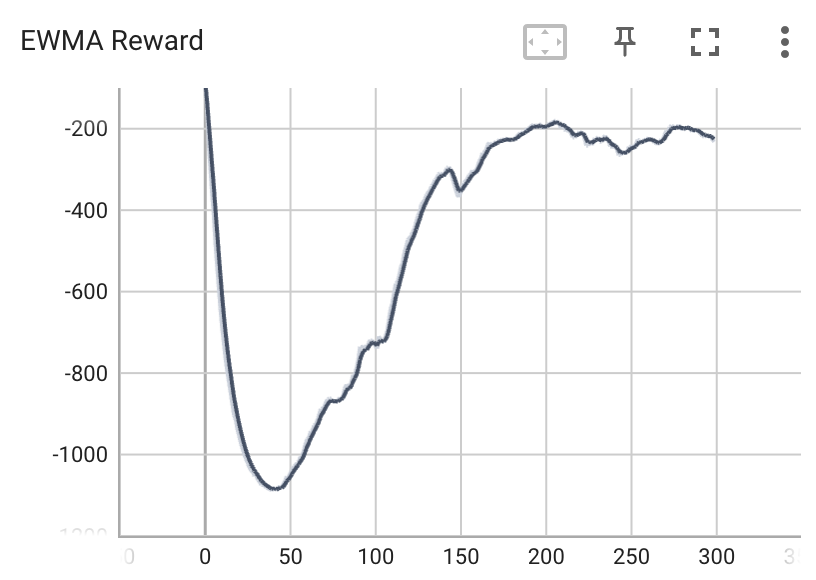
\includegraphics[width=7cm]{./imgs/pendulum/ewma_rw.png}
    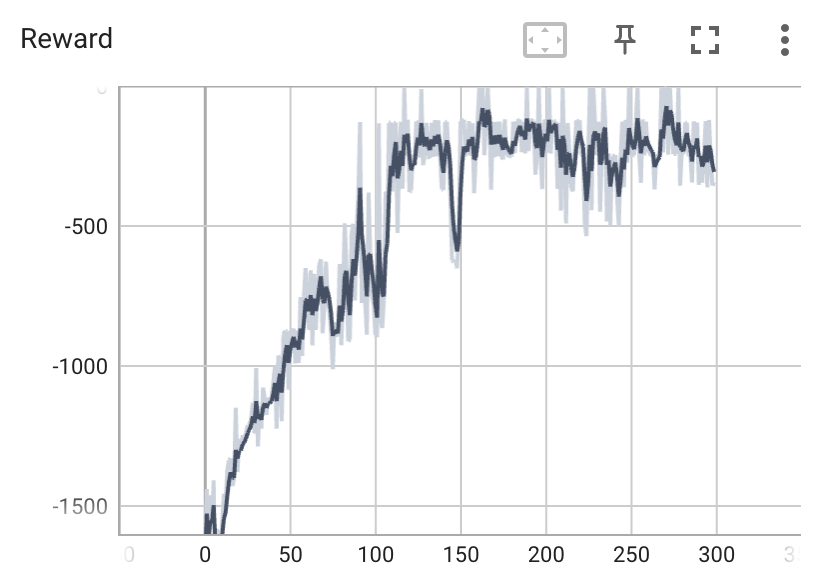
\includegraphics[width=7cm]{./imgs/pendulum/rw.png} \\
    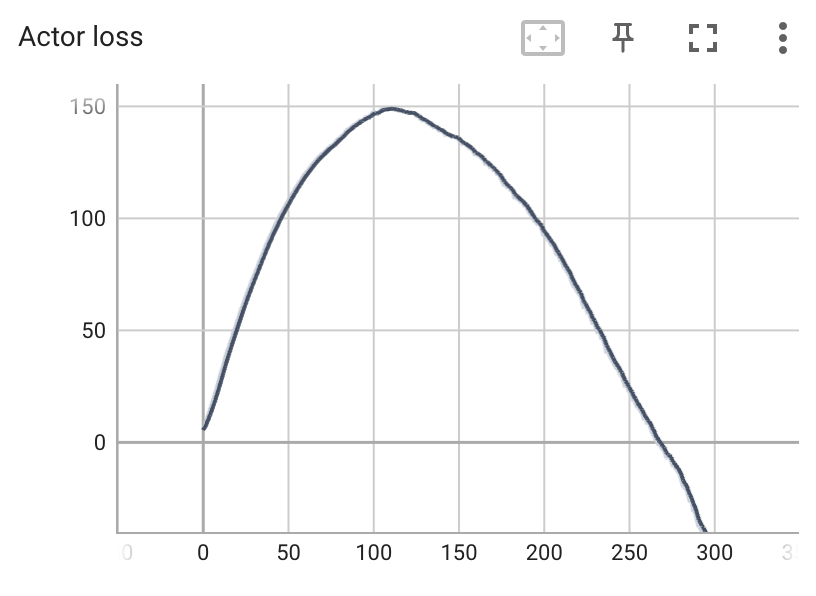
\includegraphics[width=7cm]{./imgs/pendulum/actor_loss.png}
    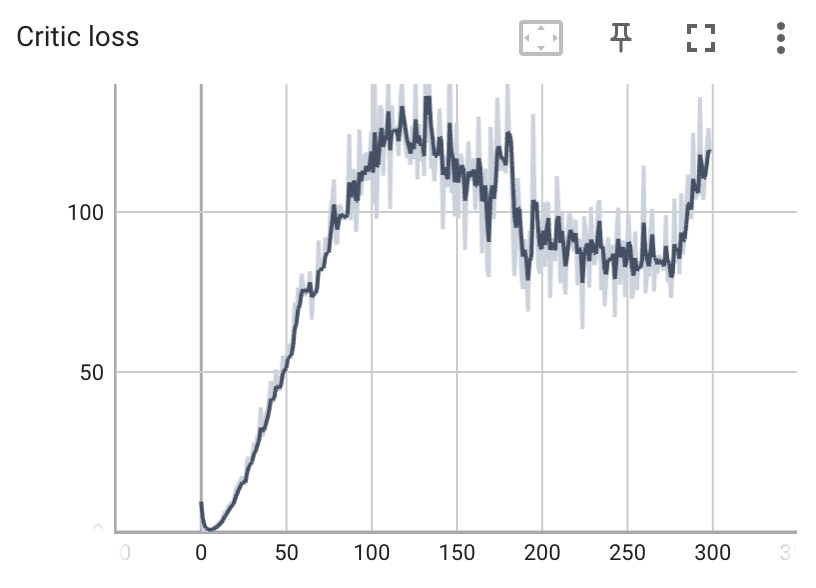
\includegraphics[width=7cm]{./imgs/pendulum/critic_loss.png}\\

    \subsection{LunarLanderContinuous-v2}
    Use bayesian optimization to tune the hyper parameters. Reach EWMA reward=120 in 616 steps.
    \begin{table}[h]
        \centering
        \begin{tabular}{|c|c|}
        \hline
        \textbf{Learning Rate(Actor)} & 0.008 \\ \hline
        \textbf{Learning Rate(Critic)} & 0.001 \\ \hline
        \textbf{Learning Rate decay rate(Actor)} & 0.85 \\ \hline
        \textbf{Learning Rate decay rate(Critic)} & 0.81 \\ \hline
        \textbf{Batch Size} & 211 \\ \hline
        \textbf{Hidden Size} & 128 \\ \hline 
        \textbf{Layer Number} & 2 \\ \hline
        \textbf{Noise Scale} & 0.28 \\ \hline 
        \end{tabular}
        \caption{Hyperparameters}
        \label{tab:ddpg_results}
    \end{table}
    \\
    EWMA Reward: \\
    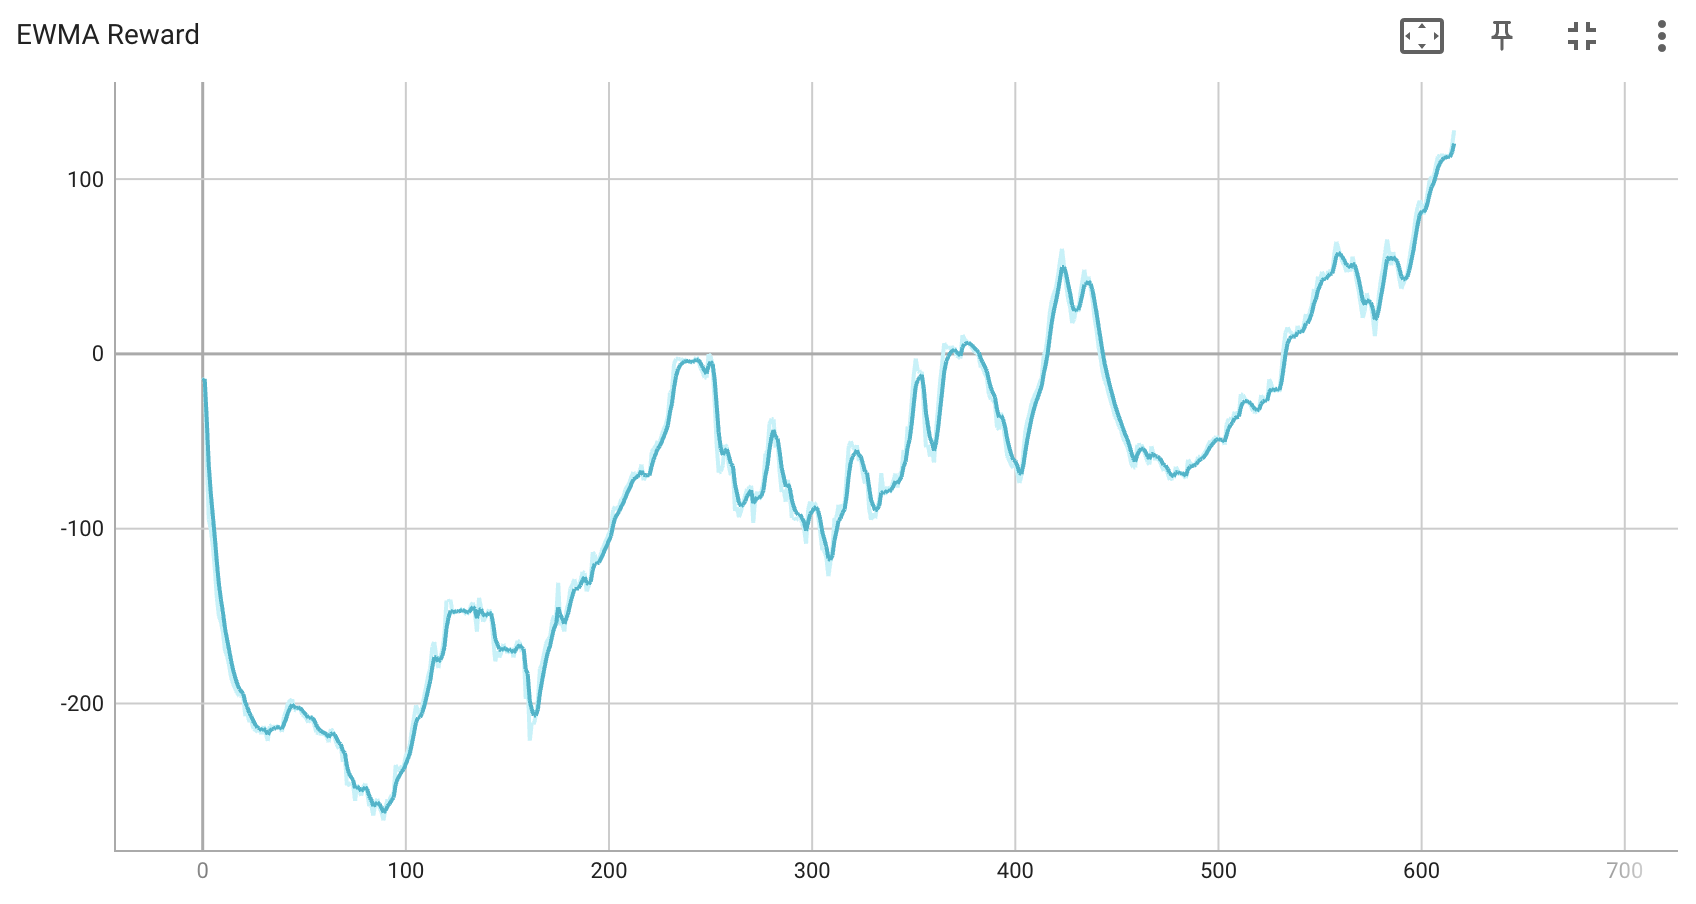
\includegraphics[width=10cm]{./imgs/lunarlander/ewma_rw.png} \\
    Reward: \\
    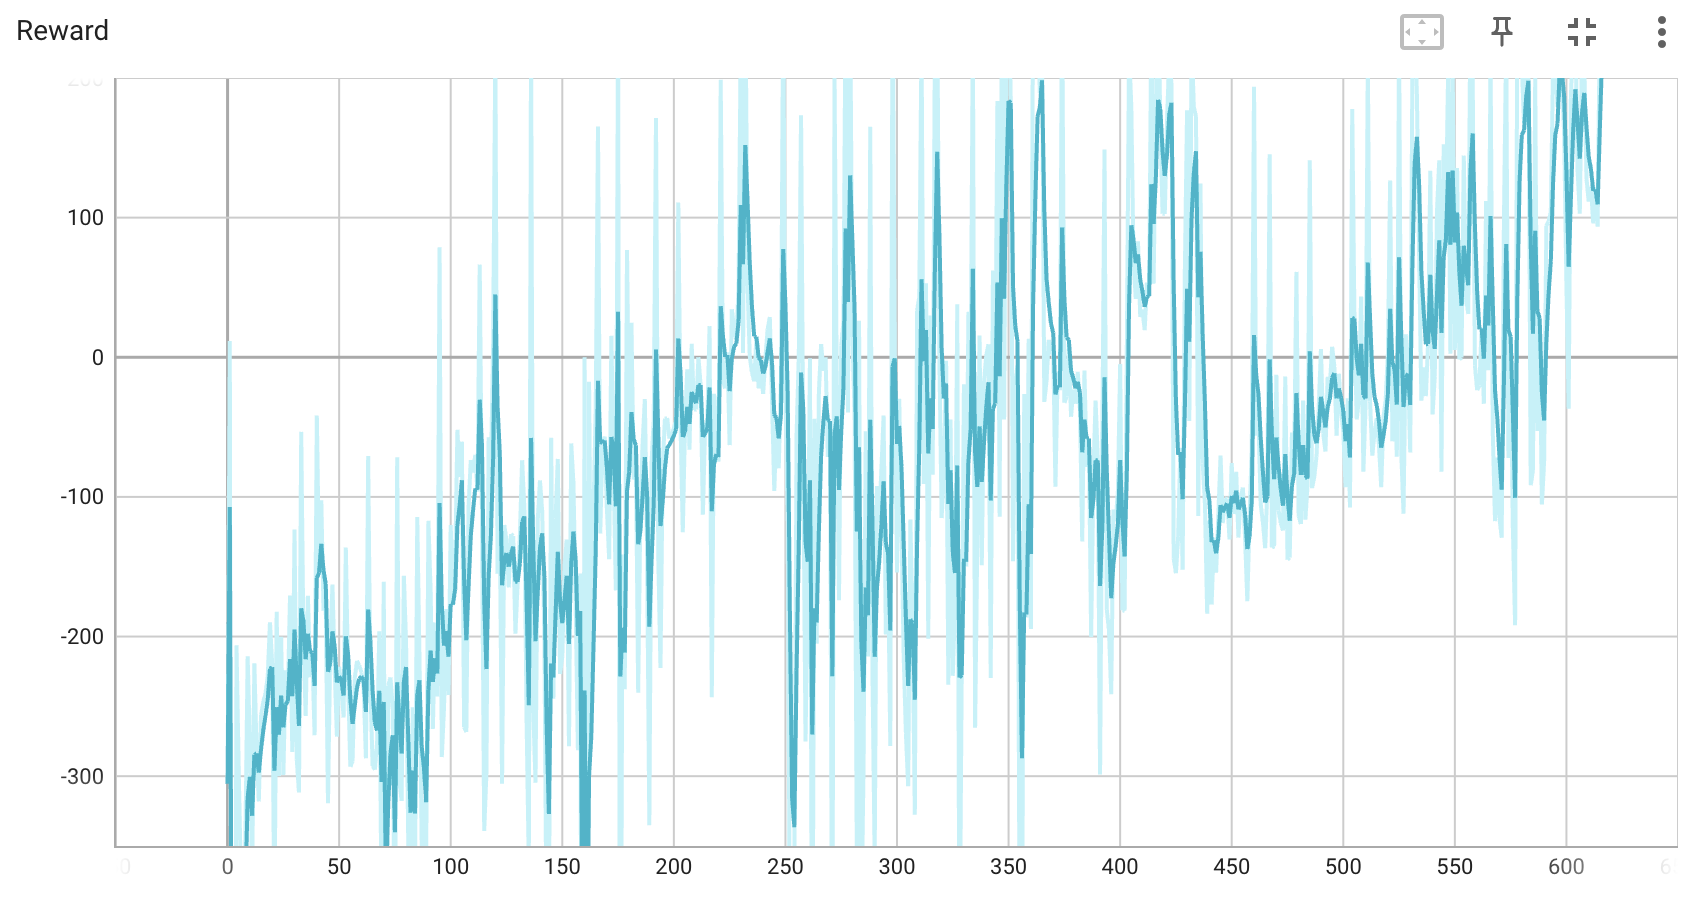
\includegraphics[width=10cm]{./imgs/lunarlander/rw.png} \\
    \\
    Loss of Actor: \\
    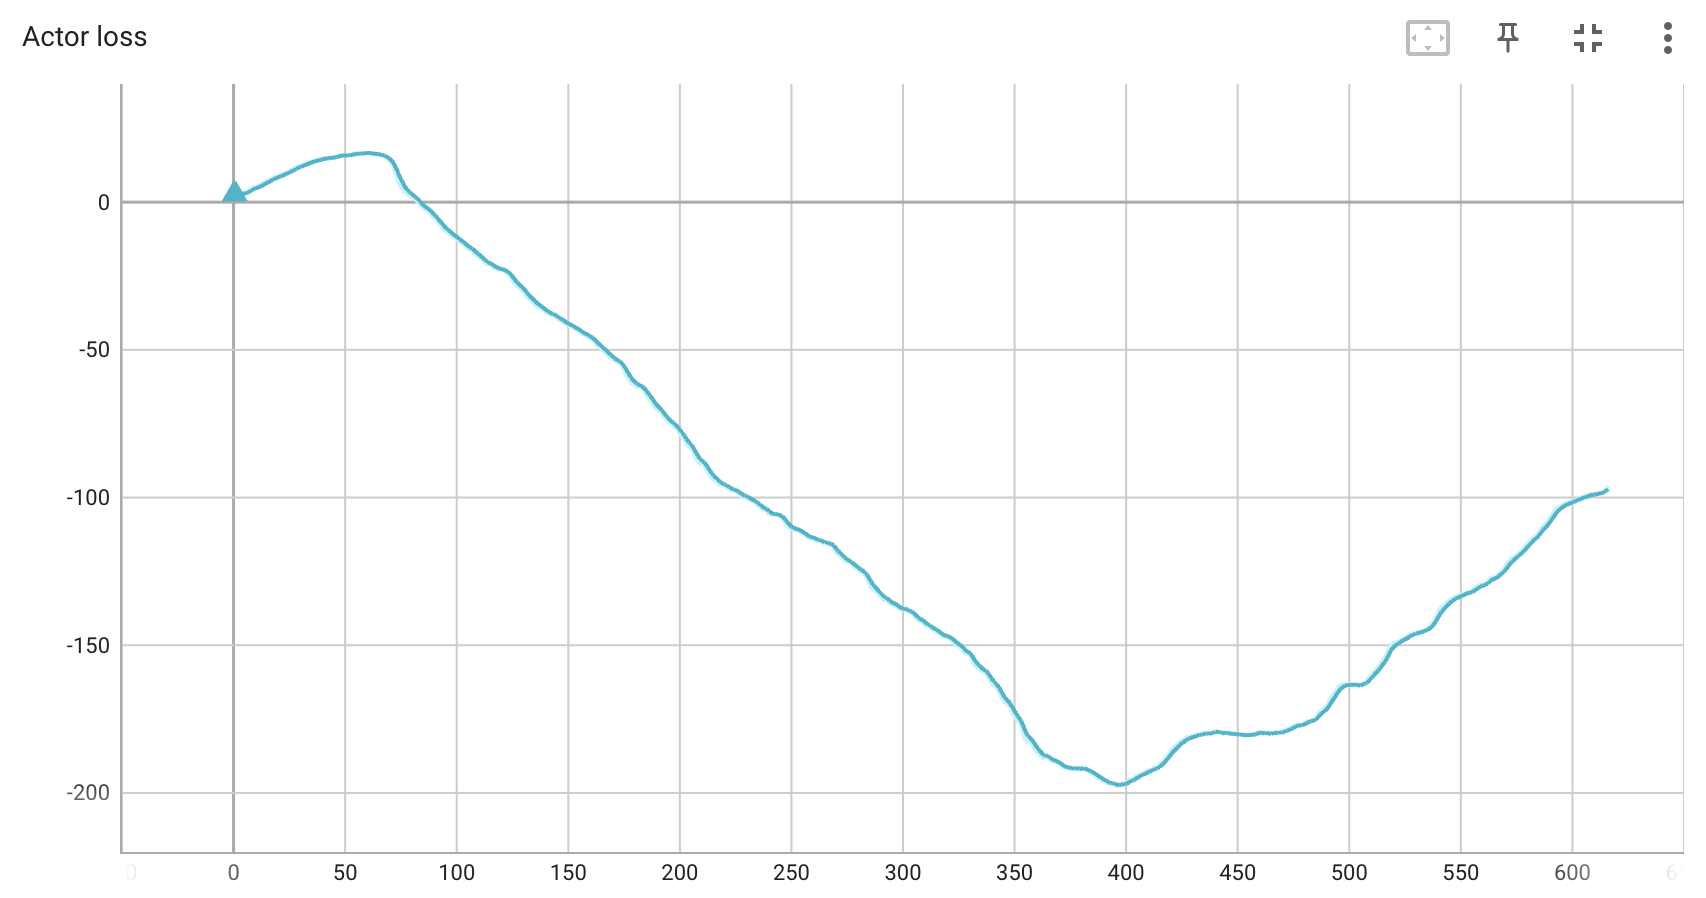
\includegraphics[width=10cm]{./imgs/lunarlander/actor_loss.png} \\
    Loss of Critic: \\
    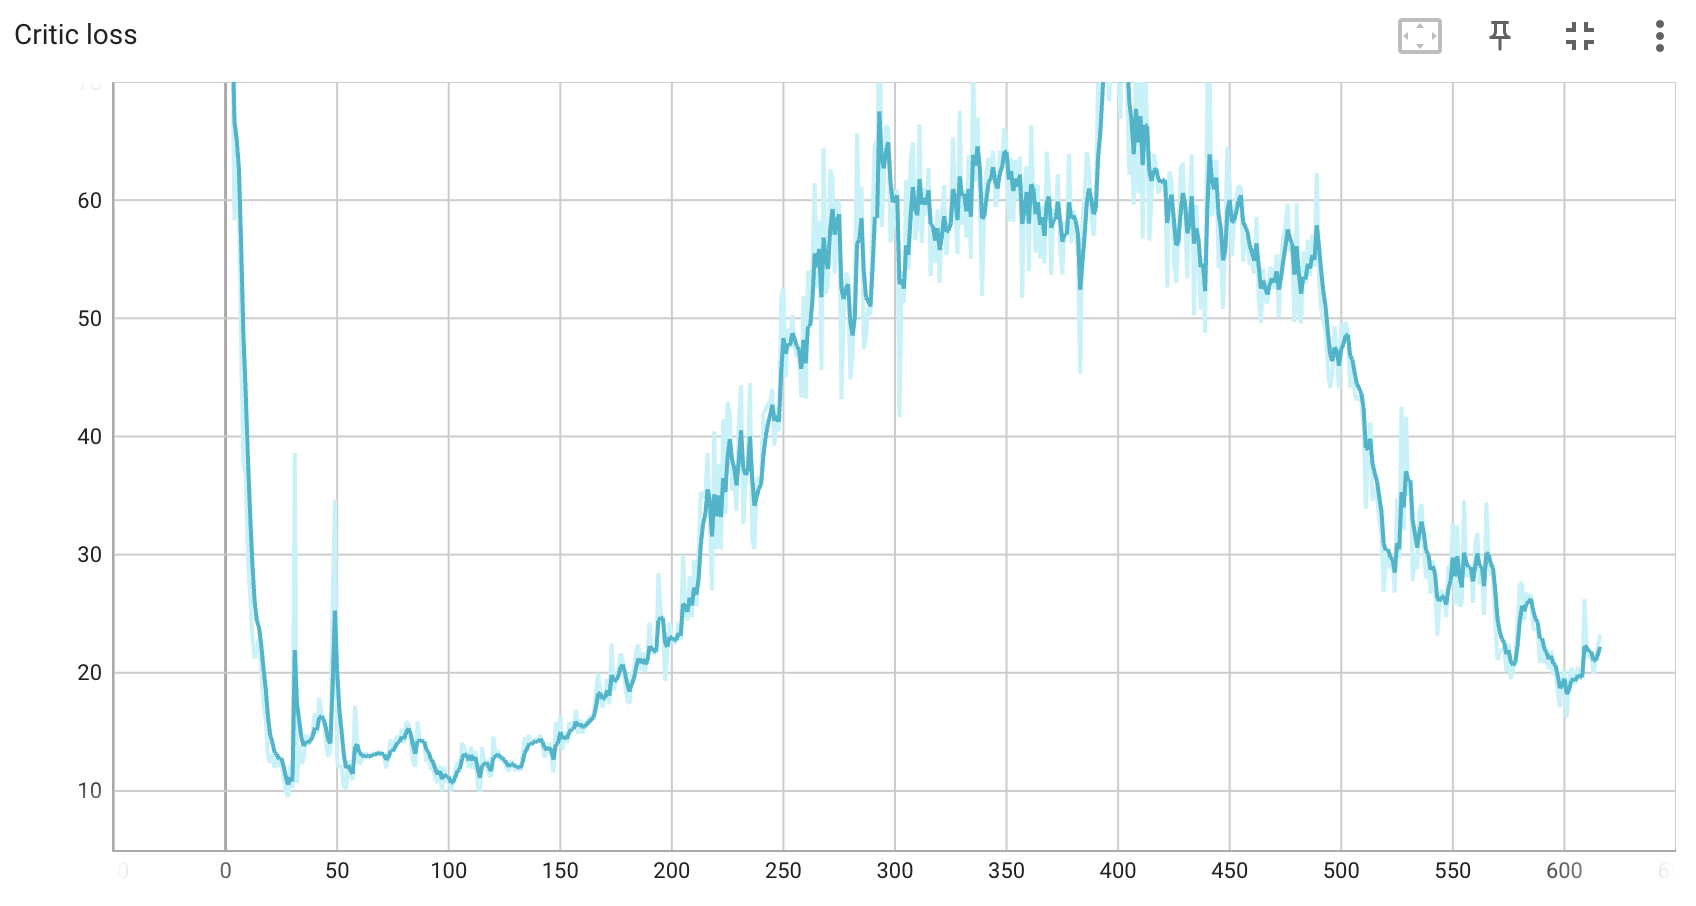
\includegraphics[width=10cm]{./imgs/lunarlander/critic_loss.png} \\
    
\end{document}